\chapter{Réseaux de neurones}

\section{Artificial Neural Network}

En 1957, un dénomé Rosenblatt Franck met au point le premier neurone électronique inspiré par son égal biologique.
L'idée qui se cache derrière le neurone est de proposer un algorithme qui apprends et s'auto-ajuste de lui-même.

\subsection{Le neurone}

Du point de vue de la machine, un neurone est un n\oe ud qui dispose d'un ensemble de signaux en entrée $x_i$ et produit un signal de sortie $y$.
Chaque lien entre un signal d'entré et notre n\oe ud est appelé \textit{synapse} et dispose d'un ``poids'' $w_i$.

\begin{figure}[ht]	
	\centering
	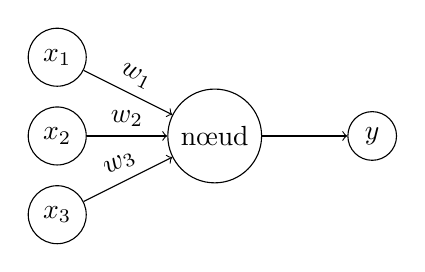
\begin{tikzpicture}
		\node[circle, draw] (n) at (2,2) {n\oe ud};
		\node[circle, draw] (y) at (4, 2) {$y$};
		\foreach \y in {1,2,3} {
			\node[circle, draw] (x-\y) at (0, 4-\y) {$x_\y$};
			\draw[->] (x-\y) -- node[sloped, above, midway] {$w_\y$} (n);
		}
		\draw[->] (n) -> (y);
	\end{tikzpicture}
	\caption{Représentation du réseau de neurone formel}
\end{figure}

Le n\oe ud fait alors une somme pondérée des signaux d'entrée par le poids de leur synapse $\sum_{i=1}^m w_i x_i$ puis utilise une fonction d'activation $\phi$ dont le résultat est envoyé par le signal de sortie $y$.

\begin{equation}
	y = \phi\left(\sum_{i=1}^m w_i x_i \right)
\end{equation}

Dans sa conception, la fonction d'activation permet de reproduire le potentiel d'activation que l'on retrouve dans le domaine de la biologie du cerveau humain. Il s'agit de l'étape qui détermine ou non la transmission de l'information. Grossièrement, il s'agit de dire si oui ou non le neurone s'active.

\paragraph{Fonction d'activation}
Nous pouvons citer les fonctions d'activation les plus répandues : \textit{la fonction seuil}, \textit{la fonction sigmo\"ide}, \textit{la fonction tanh}, \textit{la fonction redresseur}, etc.
\begin{equation}
	\phi_\text{seuil}(x) =
	\begin{cases}
		1 \text{ si } x \geq 0 \\
		0 \text{ si } x < 0
	\end{cases} \qquad
	\phi_\text{redresseur}(x) = \max(x, 0)
\end{equation}
\begin{equation}
	\phi_\text{sigmo\"ide}(x) = \frac{1}{1+\exp(-x)} \qquad
	\phi_\text{tanh}(x) = \frac{1-\exp(-2x)}{1+\exp(-2x)}
\end{equation}

\paragraph{Phase d'apprentissage}
Au cours de son entraînement, nous donnons à notre neurone un vecteur d'entrés $x$ de taille $m$ pour obtenir un résultat $\hat y$.
Nous faisons par la suite une comparaison entre la valeur souhaité $y$ et la valeur obtenue $\hat y$ à l'aide d'une fonction de coût $C$.
Ici l'équation~\ref{eq:cost_function_1} est un exemple de fonction utilisé dans des réseaux de neurones.

\begin{equation}
	\label{eq:cost_function_1} C = \frac{1}{2}(y-\hat y)^2
\end{equation}

L'objectif est de minimiser cette fonction de coût $C$ dont la valeur sert à ajuster les ``poids'' $w$ sur les différents synapses.
\begin{figure}[ht]	
	\centering
	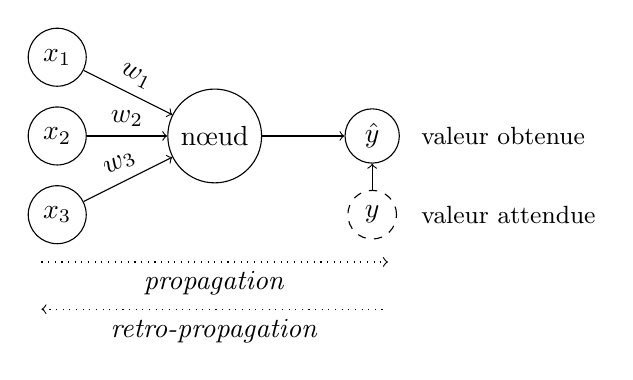
\begin{tikzpicture}
		\node[circle, draw] (n) at (2,2) {n\oe ud};
		\node[circle, draw] (y) at (4, 2) {$\hat y$};
		\node[circle, draw, dashed] (y2) at (4, 1) {$y$};
		\node[right=.5cm] at (y) {\small valeur obtenue};
		\node[right=.5cm] at (y2) {\small valeur attendue};
		\draw[->] (y2) -- (y);

		\foreach \y in {1,2,3} {
			\node[circle, draw] (x-\y) at (0, 4-\y) {$x_\y$};
			\draw[->] (x-\y) -- node[sloped, above, midway] {$w_\y$} (n);
		}
		\draw[->] (n) -> (y);

		\draw[->, dotted] (-.2, .4) -- node[midway, below] {\textit{propagation}} (4.2, .4);
		\draw[<-, dotted] (-.2, -.2) -- node[midway, below] {\textit{retro-propagation}} (4.2, -.2);
	\end{tikzpicture}
	\caption{Représentation du réseau de neurone formel}
\end{figure}
Lorsque les données parcourent le réseau de neurones de gauche à droite on parle alors de \textit{propagation}.
Tandis que lors de l'ajustement des poids, les données remontent le réseau de neurones de droite à gauche et nous parlons alors de \textit{retro-propagation}.

\paragraph{Fonction Co\^ut}

Comme nous venons de le voir, le fonction co\^ut joue un r\^ole important lors de l'apprentissage du neurone.
Il en existe plusieurs, chacunes ayant des avantages et inconvénients, certaines sont orientés sur des calculs de distribution tandis que d'autres sont plus efficaces sur des calculs de zones. Nous allons aborder certaines fonctions de manière non-exhaustives :

\subparagraph{Binary Cross-Entropy} Cette fonction mesure la différence entre deux probabilité de distribution pour une variable prise aléatoirement.

\begin{equation}
	C_p (q) = - \frac{1}{N} \sum_{i=1}^{N} y_i \log(p(y_i)) + (1 - y_i)\log(1-p(y_i))
\end{equation}

\subparagraph{Categorical Cross-Entropy}

\begin{equation}
	C = - \sum_{i = 1}^{C} t_i \log(f(s)_i)
\end{equation}

\subparagraph{Weighted Cross-Entropy}

\subparagraph{Soft Dice}

\subparagraph{Pixel-Wise Cross-Entropy}

\subparagraph{Lovasz Hinge}

\paragraph{Algorithme du gradient}
Calcul de la dérivé d'une fonction pour en trouver un résultat optimal

\subparagraph{Algorithme du gradient stochastique}
Au lieu de reévaluer les poids pour un epoch donné, l'algorithme du gradient stochastique va les modifier dès la première évaluation et ainsi de suite.

\subsection{Conception d'un réseau de neurones}
Dans cette partie, nous allons mettre en \oe uvre un \gls{ANN} à l'aide de python.

